\documentclass[a4paper,11pt]{article}
%@@@@@@@@@@@@@@@@@@@@@@@@@@@@@@@@@@@@@@@@@@@@@@@@@@@@@@@@@@@
%@@@@@@@@@@@@@@@@      PACOTES BÁSICOS		     @@@@@@@@@@
%@@@@@@@@@@@@@@@@@@@@@@@@@@@@@@@@@@@@@@@@@@@@@@@@@@@@@@@@@@@

\usepackage[T1]{fontenc}
\usepackage[utf8]{inputenc}
\usepackage{lmodern} 
\usepackage[portuguese]{babel}
\usepackage{amsmath}
\usepackage{array}
\usepackage{graphicx}				%para imagens
\usepackage{epstopdf} 				%resolve problemas eps-pdf
\usepackage{pict2e}				%%writting to images
%@@@@@@@@@@@@@@@@@@@@@@@@@@@@@@@@@@@@@@@@@@@@@@@@@@@@@@@@@@@
%@@@@@@@@@@@@@@@@     PACOTES NÃO TAOBÁSICOS		 @@@@@@@@@@
%@@@@@@@@@@@@@@@@@@@@@@@@@@@@@@@@@@@@@@@@@@@@@@@@@@@@@@@@@@@
\usepackage{fancyhdr}				% para o cabeçalho bonito
\usepackage{caption}					%para legendas
\usepackage{subcaption}				% e sublegendas
\usepackage{placeins} 				%controlar o lugar dos floats
\pagestyle{fancy} 					% número de pag e cabeçalho
\usepackage{txfonts} 				%fontes bonitas? acho que para o título
\usepackage[usenames]{color} 		% algo com gunplot e eps
\usepackage{ifthen}
\usepackage{xparse}
\graphicspath{{./../images/}{./../data/}{./graph/}}	% procura imagens nessa pasta
\usepackage{float} %%para definir ambiente gráfico
\newfloat{Gráfico}{hbtp}{lop}[section]
%\usepackage{undertilde}	%%para notação de vetor do yuri
\usepackage[import]{xy} % para escrever em imagens
\xyoption{import}

\usepackage{listings}
\lstset{frame=single,}
%@@@@@@@@@@@@@@@@@@@@@@@@@@@@@@@@@@@@@@@@@@@@@@@@@@@@@@@@@@@
%@@@@@@@@@@@@@@@@      Cabeçalho de cada página      @@@@@@@
%@@@@@@@@@@@@@@@@@@@@@@@@@@@@@@@@@@@@@@@@@@@@@@@@@@@@@@@@@@@
\setlength{\headheight}{25pt}%compila sem erro
	\fancyhead{}
	\fancyfoot{}
	\fancyhead[R]{Sistemas de Medição}%direito superior
	\fancyhead[L]{
\includegraphics[height=0.25in]{./../images/logo_unb.pdf}}%esquerda superior
	\fancyfoot[C]{\thepage}%baixo centro
%E: Even page, O: Odd page, L: Left field, C: Center field, R: Right field, H: Header, F: Footer
% em documentos com dois lados use LO, RO. como esse documento não tem lados essa opção é inútil


%@@@@@@@@@@@@@@@@@@@@@@@@@@@@@@@@@@@@@@@@@@@@@@@@@@@@@@@@@@@
%@@@@@@@@@@@@@@@@      NOVOS COMANDOS		      @@@@@@@@@
%@@@@@@@@@@@@@@@@@@@@@@@@@@@@@@@@@@@@@@@@@@@@@@@@@@@@@@@@@@@
\newcommand\undermat[2]
	{
	  \makebox[0pt][l]
	  	{$\smash{\underbrace{\phantom{%
    \begin{matrix}#2\end{matrix}}}_{\text{$#1$}}}$
    		}#2
    	}
    	
\newcommand{\HRule}
	{
	\rule{\linewidth}{0.5mm}
	}
	
\newcommand{\EmptyPage}
	{
	\thispagestyle{empty}
	\mbox{ }
	\newpage	
	} 
	
\newcommand{\MakeMyTitlePage}[4]
%%Argumentos: 
%1º Nome da Matéria
%2º subtítulo ex: experimento IV
%3º título
%4º autores
% exemplo de autores:
%	\begin{center} \large
%		\begin{tabular}{llr} \
%		& & \\[0.05cm]		
%		Professora & Nadia Maria de Liz Koche & \\
%		
%		Alunos:& & \\
%		& Juarez A.S.F 					& 11/0032829\\
%		& Sérgio Fernandes da Silva Reis & 11/0140257\\
%		& Jedhai Pimentel				& 09/0007883\\	[0.05cm]	
%		\end{tabular}
%	\end{center}
{
\begin{titlepage}
\begin{center}

% Upper part of the page. The '~' is needed because \\
% only works if a paragraph has started.

\includegraphics[width=\textwidth]{./../images/logo_unb.pdf}~\\[1cm]

\Huge #1\\[0.5cm]

\huge #2

% Title
\HRule \\[0.4cm]
{ \huge \bfseries  #3}\\[0.4cm]

\HRule \\[0.5cm]

{\large \today}


\vfill %%o que vier depois vai ao fim da páginda


%Autor e Professor
\begin{center} \large
#4
\end{center}

\end{center}
\end{titlepage}

\EmptyPage
\tableofcontents
\newpage

}
	
%@@@@@@@@@@@@@@@@@@@@@@@@@@@@@@@@@@@@@@@@@@@@@@@@@@@@@@@@@@@
%@@@@@@@@@@@@@@@@      NOVOS AMBIENTES		      @@@@@@@@@
%@@@@@@@@@@@@@@@@@@@@@@@@@@@@@@@@@@@@@@@@@@@@@@@@@@@@@@@@@@@
\newcounter{graph-c}
\setcounter{graph-c}{0}


%\NewDocumentEnvironment{Graph}{m}
 % {%antes
  %\addtocounter{graph-c}{1}
  %\begin{figure}
  %}
 %{
 %depois
%	\end{figure} 
%	\caption*{Grafico \arabic{graph-c} - #1}
 %}

















%inclui todosos pacotes utilizados

\newcommand{\MyBox}[1]
{
	\begin{tabular}{|l|}\hline
	  #1 \\ \hline	    
	\end{tabular} 	
}

\begin{document}



\MakeMyTitlePage
{Física Experimental 4}
{Experimento VI-b}
{Medida da velocidade da luz}
{%autores
		\begin{tabular}{llr} \
		& & \\[0.05cm]		
		Professora & Nadia Maria de Liz Koche & \\
		
		Alunos:& & \\
		& Juarez A.S.F 					& 11/0032829\\
		& Sérgio Fernandes da Silva Reis & 11/0140257\\
		& Jedhai Pimentel				& 09/0007883\\
	[0.05cm]	
		\end{tabular}
}

%@@@@@@@@@@@@@@@@@@@@@@@@@@@@@@@@@@@@@@@@@@@@@@@@@@@@@@@@@@@
%@@@@@@@@@@@@@@@@      OBJETIVOS      @@@@@@@@@@@@@@@@@@@@@@
%@@@@@@@@@@@@@@@@@@@@@@@@@@@@@@@@@@@@@@@@@@@@@@@@@@@@@@@@@@@
\section{Objetivos}
\paragraph{}Medir a velocidade da luz. 
%@@@@@@@@@@@@@@@@@@@@@@@@@@@@@@@@@@@@@@@@@@@@@@@@@@@@@@@@@@@
%@@@@@@@@@@@@@@@        MATERIAIS         @@@@@@@@@@@@@@@@@@
%@@@@@@@@@@@@@@@@@@@@@@@@@@@@@@@@@@@@@@@@@@@@@@@@@@@@@@@@@@@
\section{Materiais}
\paragraph{} Para o experimento utilizou-se:
\begin{itemize}
  \item fonte de laser 
  \item 2 lentes convergentes: uma de foco 50mm e outra de
    200mm 
  \item banco ótico
  \item espelho rotativo com controle de velocidade
  \item microscópio acoplado com micrômetro
  \item divisor de feixe(Beam Splitter)
  \item espelho esférico
\end{itemize}
%@@@@@@@@@@@@@@@@@@@@@@@@@@@@@@@@@@@@@@@@@@@@@@@@@@@@@@@@@@@
%@@@@@@@@@@@@@@        INTRODUCAO       @@@@@@@@@@@@@@@@@@@@ %@@@@@@@@@@@@@@@@@@@@@@@@@@@@@@@@@@@@@@@@@@@@@@@@@@@@@@@@@@@
\newpage
\section{Introdução}

\paragraph{}A velocidade da luz c é uma das propriedades mais
importante da natureza. Segundo a teoria da relatividade
ela impõe restrições para a velocidade que um corpo pode
atingir e, além disso, contra todas as intuições e princípios
da física clássica, deve ser a mesma independente do
referencial sob o qual é medida. Isso quer dizer, por
exemplo, que independente da velocidade que um observador
possua ele sempre irá ver a luz de sua lanterna de afastar
de si com a mesma velocidade. Esse fato contaria uma noção
comum que de que um jogador pode sempre lançar uma bola mais
rápida se ele realizar o mesmo lançamento enquanto corre,
acrescentando assim sua velocidade a velocidade com que seus
braços conseguem mandar a bola. Esse princípio de constância
da velocidade da luz tem várias consequências, dentre elas a
contração do espaço e do tempo. Felizmente tais previsões só
alteram significativamente os resultados clássicos em
velocidades da ordem de c e , como veremos, essas
velocidades não ocorrem no dia a dia.

\paragraph{} Os sentidos humanos não são capazes de perceber
a velocidade da luz, de modo que a luz parece se propagar
instantaneamente. Experimentos que tentam medir a velocidade
da luz do modo como normalmente medimos velocidade, ou seja,
usando $v = \frac{\triangle s}{\triangle t}$, são difíceis de
serem realizados pois para as distâncias disponíveis na
Terra o incremento de tempo dificilmente pode ser medido.
Tome por exemplo o diâmetro da Terra aproximadamente $12.74
\cdot 10^6$m, para a velocidade da luz aceita como correta a
luz demoraria apenas 0.042 segundos para percorrê-lo. Fica
claro que tal medida se torna inviável. Um modo de medir a
velocidade seria usando medidas astronômicas ou, como
faremos nesse experimento, usando resultados simples da
ótica geométrica.

\paragraph{}Considere um sistema ótico de dois espelhos e
uma fonte pontual de luz. Um dos espelhos é fixo e o outro
tem sua posição fixada mas é livre para girar em torno de
seu eixo. O sistema é posto de forma que a luz incida no
espelho rotativo, seja refletida na direção do espelho
fixo, reflita no espelho fixo e retorne ao rotativo. É de se
esperar que se o espelho rotativo for posto para rodar que o
raio que retorna do espelho fixo incida do rotativo com
ângulo de incidência diferente daquele com que o raio que
veio da fonte o incidiu inicialmente. A diferença nesse
ângulo de incidência está relacionada com o tempo que a luz
demorou para ir ao espelho fixo e retornar ao rotativo.
Conhecendo-se a velocidade com que o espelho gira e as
distâncias envolvidas pode-se determinar a velocidade da
luz. Medir esses ângulos de incidência é impraticável, mas o
exemplo ilustra como um sistema ótico pode ser usado para
medir a velocidade.

\paragraph{} Considere a figura \ref{fig:diagrama}. Nela
temos um divisor de feixe e um microscópio que permite a
visualização de um ponto imagem cujo ponto objeto é a imagem
formada pelo espelho rotativo. A diferença nos ângulos
discutidas no parágrafo anterior irá gerar variações nas
posições em que o ponto imagem aparece no microscópio. É
essa a medida que será usada no cálculo da velocidade da
luz. Seja A a distância entre a fonte e a lente L2 da
figura, B a distância entre L2 e o espelho rotativo, D a
distância do espelho rotativo a imagem formada nele,
$\omega$ a velocidade angular, em rad/sec, de rotação do
espelho e $\triangle d'$ o deslocamento observado no
microscópio. Pode ser mostrado que essas grandezas satisfazem a
relação:

\begin{equation}
  \triangle s' = \frac{4AD^2}{c(D+B)}w
  \label{eq:LeEquation}
\end{equation}

\paragraph{}A velocidade da luz pode ser então medida
através do coeficiente angular da reta acima. 
\FloatBarrier
\begin{figure}[!htp]
  \centering 
  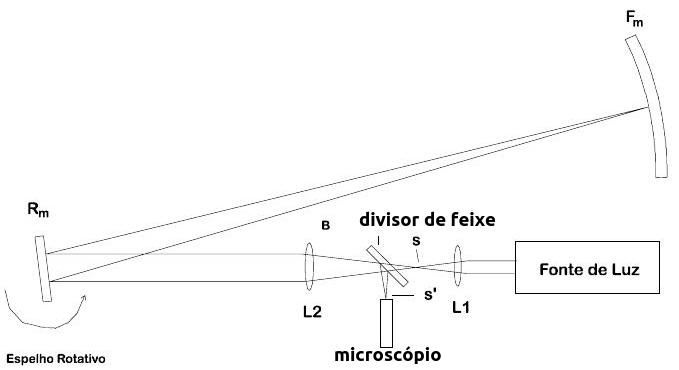
\includegraphics[scale=0.7]{./images/montagem.jpg}
  \caption{Diagrama do experimento}
  \label{fig:diagrama}
\end{figure}
\FloatBarrier

\newpage
\section{Procedimentos}
\paragraph{} A montagem é ilustrada na figura
\ref{fig:diagrama}. Inicialmente ajusta-se os espelhos de forma
a obter uma imagem nítida da fonte no microscópio.
Durante esse ajuste o espelho rotativo deve estar girando para
que o microscópio não receba a luz diretamente da fonte. Escolhe-se um 
sentido para começar as medidas e coloca-se a intensidade da rotação
em máximo. Para colocar em máximo deve-se topar o potenciômetro e apertar o 
botão vermelho do aparelho. O botão vermelho não pode ficar apertado por mais de um minuto
para não danificar o equipamento. Olhando no microscópio ajusta-se o micrômetro 
para que a divisão
horizontal coincida com a altura do ponto vermelho observado. Anota-se
a medida do micrômetro e a frequência de giro do espelho
rotativo. O procedimento é refeito para vários valores de 
frequência com valores decrescentes até que se atinja o mínimo. Agora inverte-se 
o sentido da rotação e as medidas são tomadas para valores crescentes de frequência. 
Convenciona-se um dos sentidos com positivo e o outro como negativo para 
futura análise dos dados. Devem ser medidas também as distâncias entre
as lentes L1 e L2, a distância focal de cada uma, a distância entre a lente L2
e o espelho rotativo e e a distância entre o espelho
rotativo e o espelho fixo.

\section{Dados}

\paragraph{} Os dados da posição s' em função da frequência de rotação
são mostrados na tabela \ref{tab:dataA}. Nas medidas adotamos o sentido
anti-horário como positivo.As distâncias entre os elementos e as distâncias focais são:

\begin{equation}
	\begin{array}{ll}
	A = 21.5 cm \pm  0.1 cm & \mbox{ distância entre as lentes menos a distância focal de L1} \\
	B = 40.7 cm \pm  0.1 cm & \mbox{ distância entre L2 e espelho rotativo} \\
	D = 992.00 cm \pm  0.05 cm & \mbox{ distância entre os espelhos}  \\
	F1 = +50 mm & \mbox{ distância focal de L1}  \\
	F2 = +200 mm & \mbox{ distância focal de L2}  \\	
	\end{array}
\end{equation}


\FloatBarrier
\begin{table}
\centering
	\begin{tabular}{|l|l|}\hline
	f(Hz)$\pm 1$Hz & S'(cm) $\pm 0.0005$cm \\ \hline
			 1497 &  1.0060 \\ \hline 
		 1037 &  1.0140 \\ \hline 
		 869 &  1.0155 \\ \hline 
		 703 &  1.0185 \\ \hline 
		 548 &  1.0220 \\ \hline 
		 401 &  1.0240 \\ \hline 
		 249 &  1.0255 \\ \hline 
		 111 &  1.0275 \\ \hline 
		 -111 &  1.0320 \\ \hline 
		 -258 &  1.0350 \\ \hline 
		 -402 &  1.0378 \\ \hline 
		 -555 &  1.0405 \\ \hline 
		 -699 &  1.0428 \\ \hline 
		 -856 &  1.0448 \\ \hline 
		 -1004 &  1.0485 \\ \hline 
		 -1517 &  1.0575 \\ \hline 

	\end{tabular}
\caption{posição em função da frequência}
\label{tab:dataA}
\end{table}
\FloatBarrier

\section{Análise de Dados}

\paragraph{} Os gráficos da tabela \ref{tab:dataA} são plotados na figura 
\ref{graph:A}. Não plotamos os dados puros da tabela e sim uma adaptação deles
para melhor visualização. Como aqui o que importa é o $\triangle s'$ subtraímos
de todos os dados o valor de s' na frequência mais negativa e multiplicamos por menos um para invertermos o sinal. Dessa forma temos uma reta crescente. Além disso, as frequência 
em Hz são multiplicadas por $2\pi$ para termoS a frequência angular em radianos por
segundo.

\paragraph{} A regressão linear obtida é:

\begin{equation}
	\triangle s' = (0.00000272 \pm 0.00000004)\omega+(0.0267 \pm 0.0002)

\end{equation}

O termo linear na fórmula simplesmente ajusta os dados ao nosso referencial escolhido.
O importante dessa regressão é o coeficiente angular $\alpha = (2.72 \pm 0.04)10^{-6} cm \cdot s$ que podemos comparar com a fórmula \ref{eq:LeEquation}. Usando as medidas A, B e D podemos determinar a velocidade da luz como:

\begin{equation}
	c = \frac{4AD^2 }{(D+B)\alpha} = \frac{4\cdot26.5cm\cdot(992.00 cm)^2}{(1032.7 cm)
	\cdot (0.00000272 cm \cdot s)} = 3.01285836 \cdot 10^{10} \frac{cm}{s}
\end{equation}

vamos aproximar o erro. Para facilitar as contas vamos considerar $(E = D + B = 1032.7 \pm 0.2)cm$ uma variável independente. Nesse caso o erro pode ser aproximado como:

\begin{equation}
	|\triangle c| \leq 4\left[ |\frac{D^2}{E \alpha}\triangle A|
	+|\frac{A2D}{E \alpha}\triangle D| +
	|\frac{AD^2 (-1)}{E^2 \alpha}\triangle E |+
	|\frac{AD^2 (-1)}{E \alpha^2}\triangle \alpha |\right] 
\end{equation}

\begin{equation}
	|\triangle c| \leq (1.4 \cdot 10^{8}
	+ 3.0 \cdot 10^{6}
	+ 7.2 \cdot 10^{6}
	+ 1.4 \cdot 10^{8}) \frac{cm}{s}
\end{equation}

e o erro total é:
\begin{equation}
	|\triangle c| = (3 \cdot 10^{8})cm/S
\end{equation}

Portanto nossa medida foi:

\begin{equation}
\MyBox{$	c = (3.01 \pm 0.03) \cdot 10^{10} \frac{cm}{s}$}
\end{equation}



Vemos que os dois fatores que mais influenciam no erro são a distância entre a fonte 
e a lente L2 e o coeficiente angular da reta da regressão. 


\paragraph{} O valor aceito para a velocidade da luz é de $2.99796x10^{10}cm/s$. O valor 
difere do nosso por $0.012 x 10^{8}$, dentro da margem de erro encontrada e portanto
as medidas foram acuradas. Além disso a margem de erro calculada é de 1\% e o experimento
foi preciso.


\FloatBarrier
\begin{figure}
         % GNUPLOT: LaTeX picture with Postscript
\begingroup
  \fontfamily{phv}%
  \selectfont
\definecolor{t}{rgb}{0.5,0.5,0.5}
  \makeatletter
  \providecommand\color[2][]{%
    \GenericError{(gnuplot) \space\space\space\@spaces}{%
      Package color not loaded in conjunction with
      terminal option `colourtext'%
    }{See the gnuplot documentation for explanation.%
    }{Either use 'blacktext' in gnuplot or load the package
      color.sty in LaTeX.}%
    \renewcommand\color[2][]{}%
  }%
  \providecommand\includegraphics[2][]{%
    \GenericError{(gnuplot) \space\space\space\@spaces}{%
      Package graphicx or graphics not loaded%
    }{See the gnuplot documentation for explanation.%
    }{The gnuplot epslatex terminal needs graphicx.sty or graphics.sty.}%
    \renewcommand\includegraphics[2][]{}%
  }%
  \providecommand\rotatebox[2]{#2}%
  \@ifundefined{ifGPcolor}{%
    \newif\ifGPcolor
    \GPcolortrue
  }{}%
  \@ifundefined{ifGPblacktext}{%
    \newif\ifGPblacktext
    \GPblacktextfalse
  }{}%
  % define a \g@addto@macro without @ in the name:
  \let\gplgaddtomacro\g@addto@macro
  % define empty templates for all commands taking text:
  \gdef\gplbacktext{}%
  \gdef\gplfronttext{}%
  \makeatother
  \ifGPblacktext
    % no textcolor at all
    \def\colorrgb#1{}%
    \def\colorgray#1{}%
  \else
    % gray or color?
    \ifGPcolor
      \def\colorrgb#1{\color[rgb]{#1}}%
      \def\colorgray#1{\color[gray]{#1}}%
      \expandafter\def\csname LTw\endcsname{\color{white}}%
      \expandafter\def\csname LTb\endcsname{\color{black}}%
      \expandafter\def\csname LTa\endcsname{\color{black}}%
      \expandafter\def\csname LT0\endcsname{\color[rgb]{1,0,0}}%
      \expandafter\def\csname LT1\endcsname{\color[rgb]{0,1,0}}%
      \expandafter\def\csname LT2\endcsname{\color[rgb]{0,0,1}}%
      \expandafter\def\csname LT3\endcsname{\color[rgb]{1,0,1}}%
      \expandafter\def\csname LT4\endcsname{\color[rgb]{0,1,1}}%
      \expandafter\def\csname LT5\endcsname{\color[rgb]{1,1,0}}%
      \expandafter\def\csname LT6\endcsname{\color[rgb]{0,0,0}}%
      \expandafter\def\csname LT7\endcsname{\color[rgb]{1,0.3,0}}%
      \expandafter\def\csname LT8\endcsname{\color[rgb]{0.5,0.5,0.5}}%
    \else
      % gray
      \def\colorrgb#1{\color{black}}%
      \def\colorgray#1{\color[gray]{#1}}%
      \expandafter\def\csname LTw\endcsname{\color{white}}%
      \expandafter\def\csname LTb\endcsname{\color{black}}%
      \expandafter\def\csname LTa\endcsname{\color{black}}%
      \expandafter\def\csname LT0\endcsname{\color{black}}%
      \expandafter\def\csname LT1\endcsname{\color{black}}%
      \expandafter\def\csname LT2\endcsname{\color{black}}%
      \expandafter\def\csname LT3\endcsname{\color{black}}%
      \expandafter\def\csname LT4\endcsname{\color{black}}%
      \expandafter\def\csname LT5\endcsname{\color{black}}%
      \expandafter\def\csname LT6\endcsname{\color{black}}%
      \expandafter\def\csname LT7\endcsname{\color{black}}%
      \expandafter\def\csname LT8\endcsname{\color{black}}%
    \fi
  \fi
  \setlength{\unitlength}{0.0500bp}%
  \begin{picture}(7936.00,5668.00)%
    \gplgaddtomacro\gplbacktext{%
      \csname LTb\endcsname%
      \put(882,576){\makebox(0,0)[r]{\strut{} 0}}%
      \put(882,1335){\makebox(0,0)[r]{\strut{} 0.01}}%
      \put(882,2093){\makebox(0,0)[r]{\strut{} 0.02}}%
      \put(882,2852){\makebox(0,0)[r]{\strut{} 0.03}}%
      \put(882,3610){\makebox(0,0)[r]{\strut{} 0.04}}%
      \put(882,4369){\makebox(0,0)[r]{\strut{} 0.05}}%
      \put(882,5127){\makebox(0,0)[r]{\strut{} 0.06}}%
      \put(990,396){\makebox(0,0){\strut{}-10000}}%
      \put(1652,396){\makebox(0,0){\strut{}-8000}}%
      \put(2314,396){\makebox(0,0){\strut{}-6000}}%
      \put(2976,396){\makebox(0,0){\strut{}-4000}}%
      \put(3638,396){\makebox(0,0){\strut{}-2000}}%
      \put(4301,396){\makebox(0,0){\strut{} 0}}%
      \put(4963,396){\makebox(0,0){\strut{} 2000}}%
      \put(5625,396){\makebox(0,0){\strut{} 4000}}%
      \put(6287,396){\makebox(0,0){\strut{} 6000}}%
      \put(6949,396){\makebox(0,0){\strut{} 8000}}%
      \put(7611,396){\makebox(0,0){\strut{} 10000}}%
      \put(144,2851){\makebox(0,0){\strut{}$\triangle s (cm)$}}%
      \put(4300,126){\makebox(0,0){\strut{}frequência(rad/s)}}%
      \put(4300,5397){\makebox(0,0){\strut{}$\triangle s$ em função da frequência}}%
    }%
    \gplgaddtomacro\gplfronttext{%
      \csname LTb\endcsname%
      \put(2178,4974){\makebox(0,0)[r]{\strut{}dados}}%
      \csname LTb\endcsname%
      \put(2178,4794){\makebox(0,0)[r]{\strut{}regressão}}%
    }%
    \gplbacktext
    \put(0,0){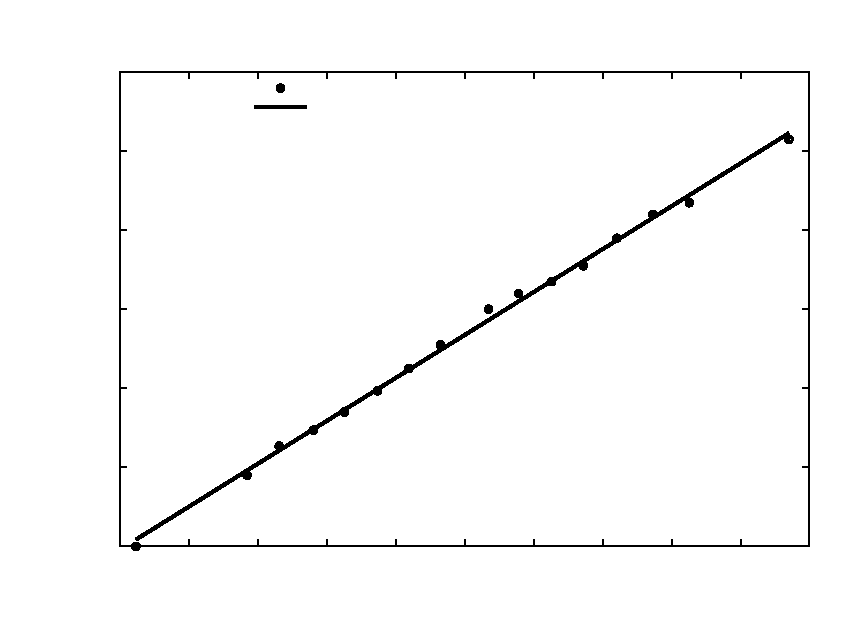
\includegraphics{./../graph/graphA}}%
    \gplfronttext
  \end{picture}%
\endgroup

        \caption{$\triangle s'$ em função de $\omega$}
        \label{graph:A}
\end{figure}
\FloatBarrier

\section{Conclusão}
\paragraph{} O experimento permitiu calcular a velocidade da luz em
 $c = (3.01 \pm 0.03)\cdot 10^{8} m/s$. A margem de erro é de 1\% da melhor
 medida e engloba o valor tabelado. O experimento foi portanto acurado e preciso.  





%@@@@@@@@@@@@@@@@@@@@@@@@@@@@@@@@@@@@@@@@@@@@@@@@@@@@@@@@@@@
%@@@@@@@@@@@@@@       REFERÊNCIAS     @@@@@@@@@@@@@@@@@@@@@@
%@@@@@@@@@@@@@@@@@@@@@@@@@@@@@@@@@@@@@@@@@@@@@@@@@@@@@@@@@@@
\begin{thebibliography}{9}    
	 \bibitem{fis4-serway}
  		JEWETT, J.W.; SERWAY, R.A.
  		\emph{Física para cientistas e engenheiros}
volume 4 : Luz, Óptica e Física Moderna.
 		 8ª ed.
 		 São Paulo : Cengage Learning, 2012.
 		 
\end{thebibliography}
\end{document}
